\documentclass[11pt,letterpaper,spanish]{article}

\usepackage{amsmath,amsthm,amssymb,amsfonts,amsxtra,amstext,anysize,graphicx}

%% Para los usuarios de windows descomentar esta linea y utilizar acentos normalmente.
\usepackage[utf8]{inputenc}
\usepackage[spanish]{babel}
\usepackage{mathrsfs}
\usepackage{fullpage}
\usepackage{verbatim}
\usepackage{graphicx}
\usepackage{subfigure}
\usepackage{wrapfig}
\usepackage{esint}
\usepackage{epsfig}
\usepackage{epstopdf}
\usepackage{multirow}
\usepackage{caption}
\usepackage{hyperref}
\usepackage{float}
\usepackage{color}
\usepackage{pdfpages}% Se utiliza para poder
%\newcommand{\parrafo}[1]{\paragraph{#1}\mbox{}\\}


%% LaTeX will automatically break titles if they run longer than
%% one line. However, you may use \\ to force a line break if
%% you desire.
\usepackage{color}
\definecolor{gray97}{gray}{.97}
\definecolor{gray75}{gray}{.75}
\definecolor{gray45}{gray}{.45}
\usepackage{listings}
\lstset{ frame=Ltb,
framerule=0pt,
aboveskip=0.5cm,
framextopmargin=3pt,
framexbottommargin=3pt,
framexleftmargin=0.4cm,
framesep=0pt,
rulesep=.4pt,
backgroundcolor=\color{gray97},
rulesepcolor=\color{black},
%
stringstyle=\ttfamily,
showstringspaces = false,
basicstyle=\small\ttfamily,
commentstyle=\color{gray45},
keywordstyle=\bfseries ,
%
numbers= none,
numbersep=15pt,
numberstyle=\tiny ,
numberfirstline = false,
breaklines=true,
}

% minimizar fragmentado de listados
\lstnewenvironment{listing}[1][]
{\lstset{#1}\pagebreak[0]}{\pagebreak[0]}

\lstdefinestyle{consola}
{
basicstyle=\scriptsize\bf\ttfamily,
backgroundcolor=\color{gray75},
}

\lstdefinestyle{C}
{language=C,
}

\begin{document} %%Comienza el documento 
\renewcommand{\tablename}{Tabla}

  
\epsfig{file= figuras/logonitido, width= 2.3 cm} %% Agrega una imagen
    \begin{tabular}{l}%% tabular va con una "l" no con un uno
    Pontificia Universidad Cat\'olica de Chile\\
    Escuela de Ingenier\'ia\\
    Departamento de Ingenier\'ia El\'ectrica\\
  \vspace{1.9 cm}\mbox{}
    \end{tabular}
    \bigskip
 
\begin{center}
\huge{Implementación de una comunicación entre un computador y un FPGA en tiempo real, por puerto USB .}\\
%\Large{\textbf{}}\\
%\normalsize{3- Sesiones}
\vspace{0.5 cm}
\hrule
\vspace{0.1 cm}
\hrule
\end{center}
\vspace{0.2 cm}
\section{Resumen}
\par 
	En este documento se presenta una guía para implementar una comunicación por el puerto USB entre un computador y una  FPGA. En particular se desarrolla una aplicación para implementar la comunicación entre una tarjeta de desarrollo Nexys 2 y un computador con sistema operativo Windows. La base de este sistema radica en la emulación de un puerto pararlelo, lo cual se lleva a cabo por medio de un microcontrolador Cypress CY7C68013A en la tarjeta, el cual se encarga de controlar la comunicación. 
	
	Para motivar el trabajo presentado se desarrolla una pequeña aplicación en la FPGA la cual permite almacenar datos provenientes desde el computador en una memoria y acceder a ellos desde los periféricos disponibles en la tarjeta. \footnote{Esta aplicación se encuentra basada en el proyecto entregado por el fabricante disponible en https://reference.digilentinc.com/digilent\_adept\_2}

\section{Introducción}
Al momento de desarrollar proyectos que involucren el trabajo con una FPGA, frecuentemente nos vemos enfrentados al problema de generar una comunicación en tiempo real con el computador, ya sea con el fin de poder \textit{debuguear}, cambiar o  configurar registros  \textit{on line}, entre otros. Para solucionar este problema existen diversos métodos que implementan distintos protocolos de comunicación. Sin embargo, en la actualidad, el protocolo USB se ha vuelto casi un estándar, siendo utilizado por un sin número de dispositivos. De hecho es muy probable que la elección de cualquier otro protocolo implique tener que adquirir un dispositivo que se encargue de traducir desde dicho protocolo a USB. 
Es por esta razón que este documento presenta una guía, en la cual se expone una implementación de una comunicación entre un computador y un puerto USB. Esta implementación fue desarrollada para un computador con sistema operativo Windows y una tarjeta de desarrollo para FPGA Nexys 2. Sin embargo la metodología para otras tecnologías es bastante similar a la propuesta.


\section{Comunicación USB}
 La comunicación por USB es un protocolo del tipo maestro/esclavo, en donde el maestro es el computador o host, mientras que el dispositivo o  periférico implementa el esclavo. De este modo, para poder realizar una correcta comunicación es necesario contar con inteligencia correcta tanto en el maestro como en el esclavo. Por otra parte, en el maestro es necesario contar con los controladores del esclavo, mientras que  en el esclavo es necesario contar con algún tipo de interprete de las señales provenientes desde el maestro. En nuestro caso particular, los drivers necesarios están disponibles en la página del distribuidor en el SDK dpcutil.dll \footnote{todos los archivos necesarios están disponibles en https//:reference.digilentinc.com/digilent\_adept\_2}, la cual implementa todas las funciones de bajo nivel para poder realizar la comunicación. En el esclavo, que en esta caso representa nuestra tarjeta Nexys 2, contamos con el integrado CYPRESS 68001A, el cual se encarga de interpretar el protocolo USB y emula un puerto paralelo (protocolo EPP\footnote{para más información revisar https://reference.digilentinc.com/\_media/dpimref\_programmers\_manual.pdf}) disponible para ser utilizado por la FPGA. De este modo, es como si la FPGA estuviera conectada a un puerto paralelo.

En resumen la tarea a realizar se compone de dos partes, la primera consiste en crear un código que se ejecute desde el computador, el cual utilice las funciones entregadas por el fabricante, que estan disponibles en la biblioteca dpcutil.dll y por otro lado crear una aplicación en la FPGA que sea capaz manejar una comunicación con el protocolo EPP.

\subsection{protocolo EPP}
El protocolo de puerto paralelo consiste físicamente en un bus bi-direccional de 8 \textit{bits} el cual sirve tanto para enviar como recibir datos, más un set de 4 señales que coordinan la dirección del flujo de datos. 


\begin{tabular}{|c|c|c|}
\hline
Señal& Detalle& Dirección \\
\hline
DB [ 7:0 ]  & Bus de datos & Bidirecciónal \\ 
\hline 
WRITE & Control de flujo de escritura & Desde el puerto paralelo emulado hacia la FPGA \\ 
\hline 
ASTB & Strobe de dirección &Desde el puerto paralelo emulado hacia la FPGA \\ 
\hline 
DSTB & Strobe de datos & Desde el puerto paralelo emulado hacia la FPGA \\ 
\hline 
WAIT & Estado del canal & Desde la FPGA hacia el puerto paralelo emulado \\ 
\hline 
\end{tabular} 
\hfill \break



Para poder implementar una interfaz en la FPGA que se comunique con el puerto paralelo es necesario contar con dos registros de 8 bits, uno de dirección y uno de datos. El registro de dirección almacena la dirección de destino para el dato a transferir. De este modo existen cuatro operaciones posibles, las cuales se muestran en las imágenes \ref{addres_read},\ref{address_write},\ref{data_read} y \ref{data_write}.


	\begin{figure}[h!]
	\begin{center}
	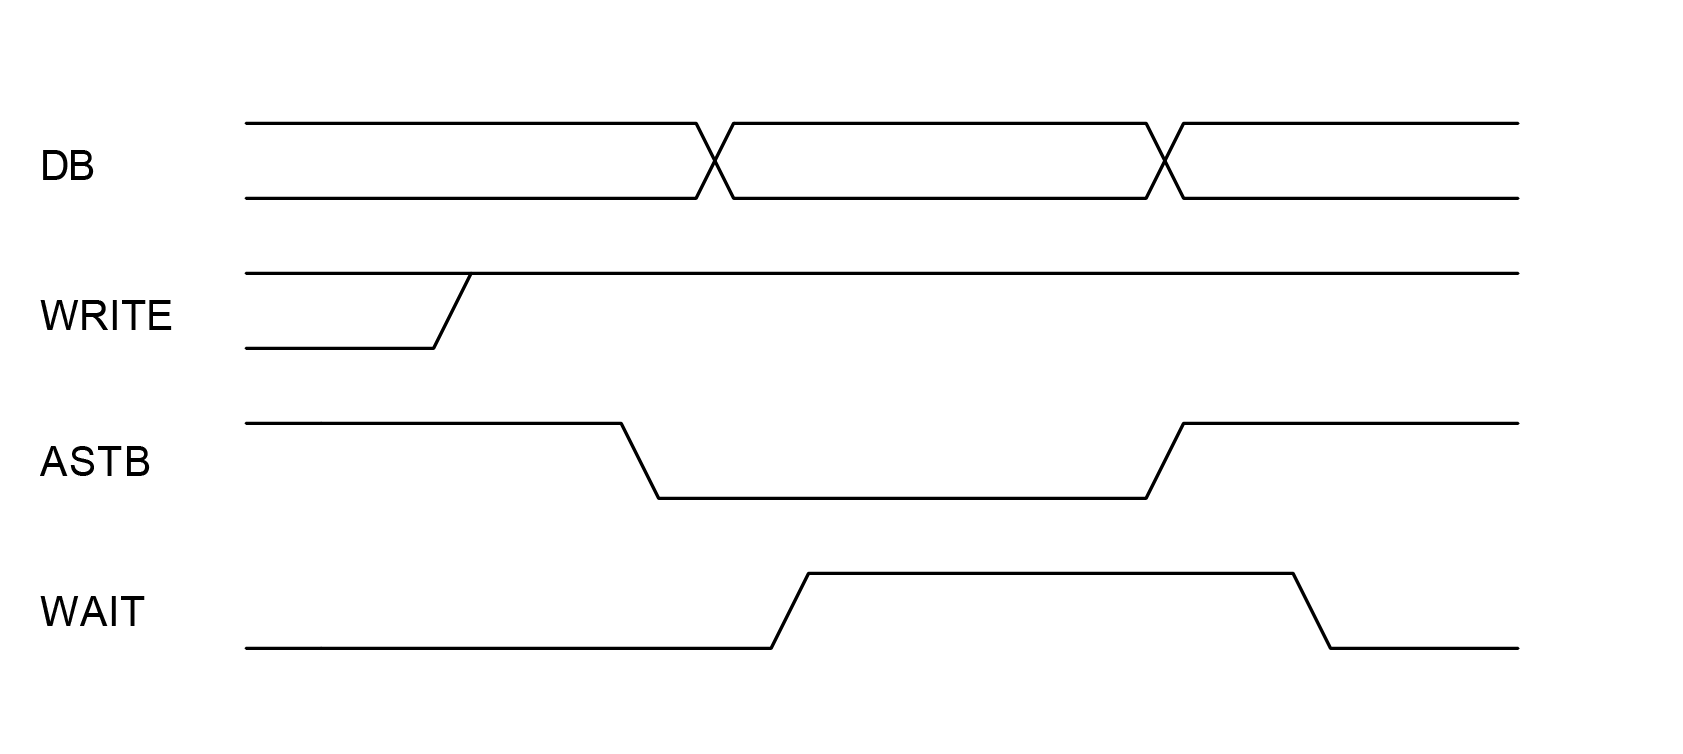
\includegraphics[width=0.4\textwidth]{figuras/address_read.png} 
	\caption{\label{addres_read} Lectura de dirección.}
	\end{center}
	\end{figure}

	\begin{figure}[h!]
	\begin{center}
	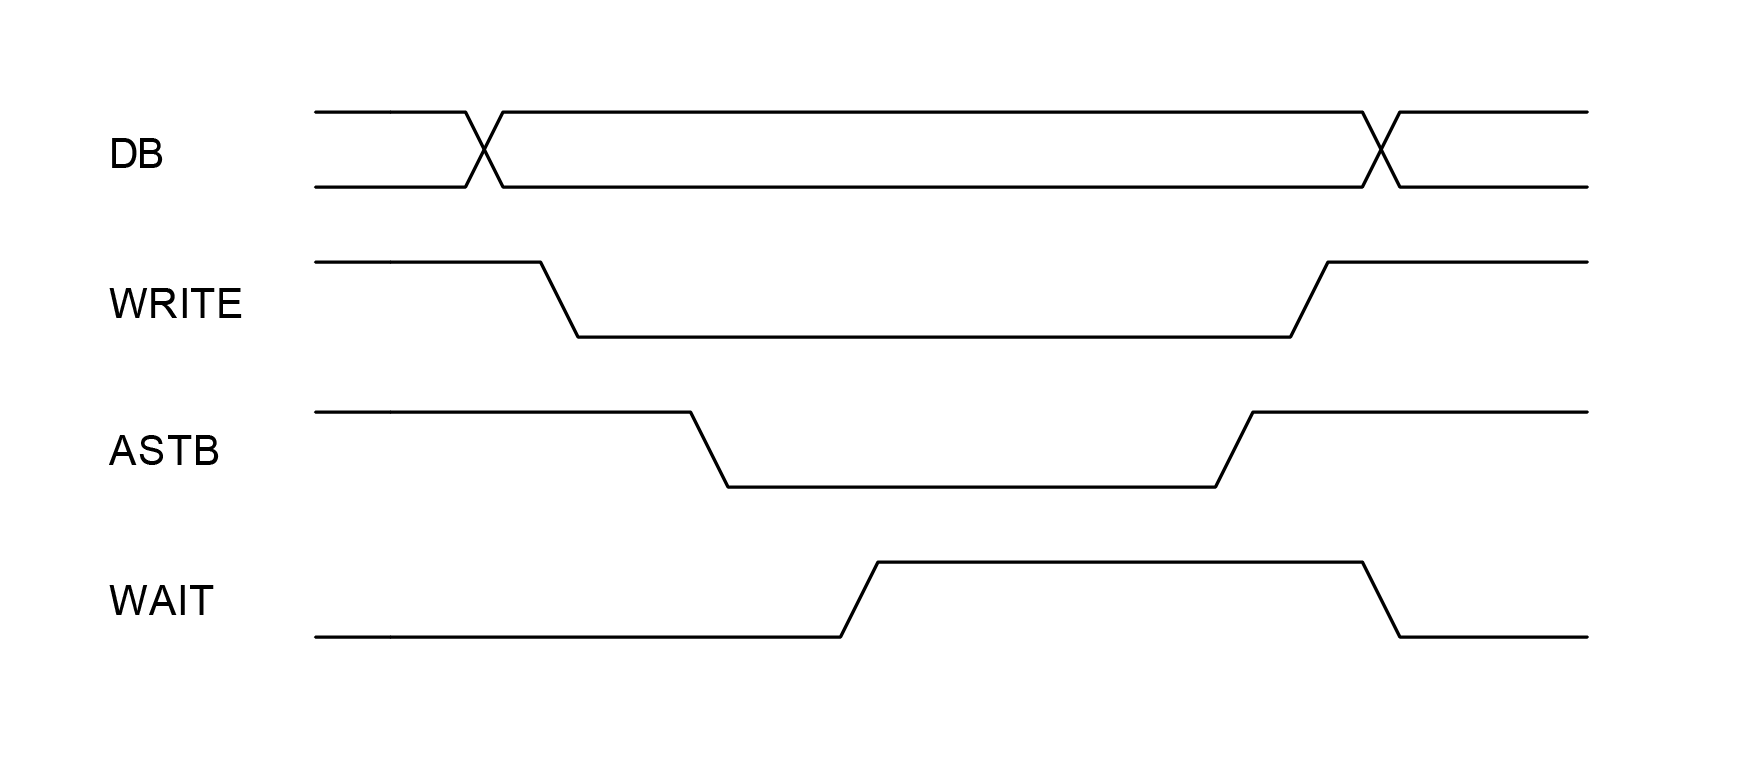
\includegraphics[width=0.4\textwidth]{figuras/address_write.png} 
	\caption{\label{address_write} Escritura de dirección.}
	\end{center}
	\end{figure}


	\begin{figure}[h!]
	\begin{center}
	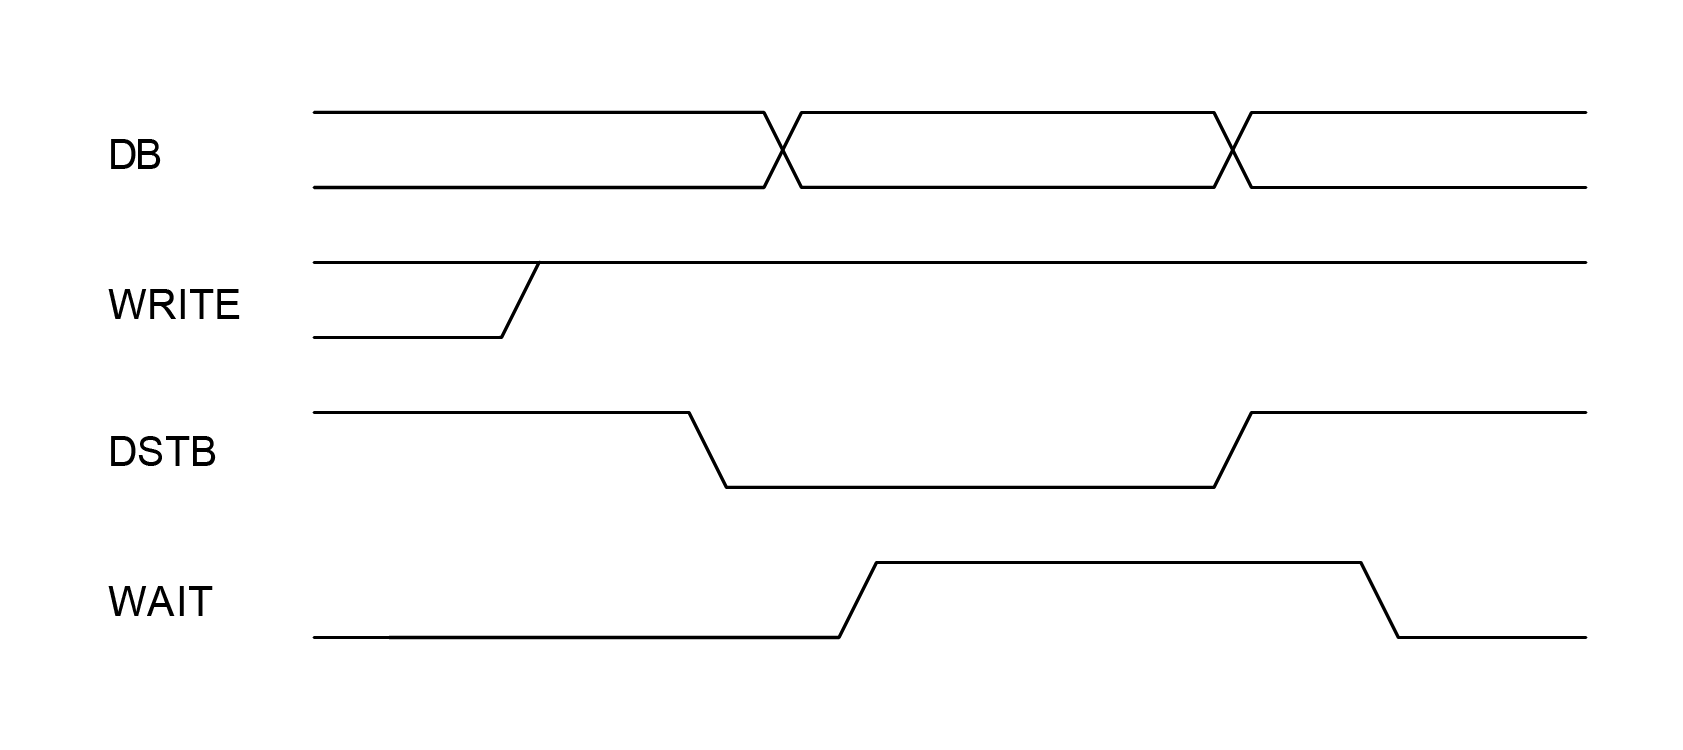
\includegraphics[width=0.4\textwidth]{figuras/data_read.png} 
	\caption{\label{data_read} Lectura de dato.}
	\end{center}
	\end{figure}

	\begin{figure}[h!]
	\begin{center}
	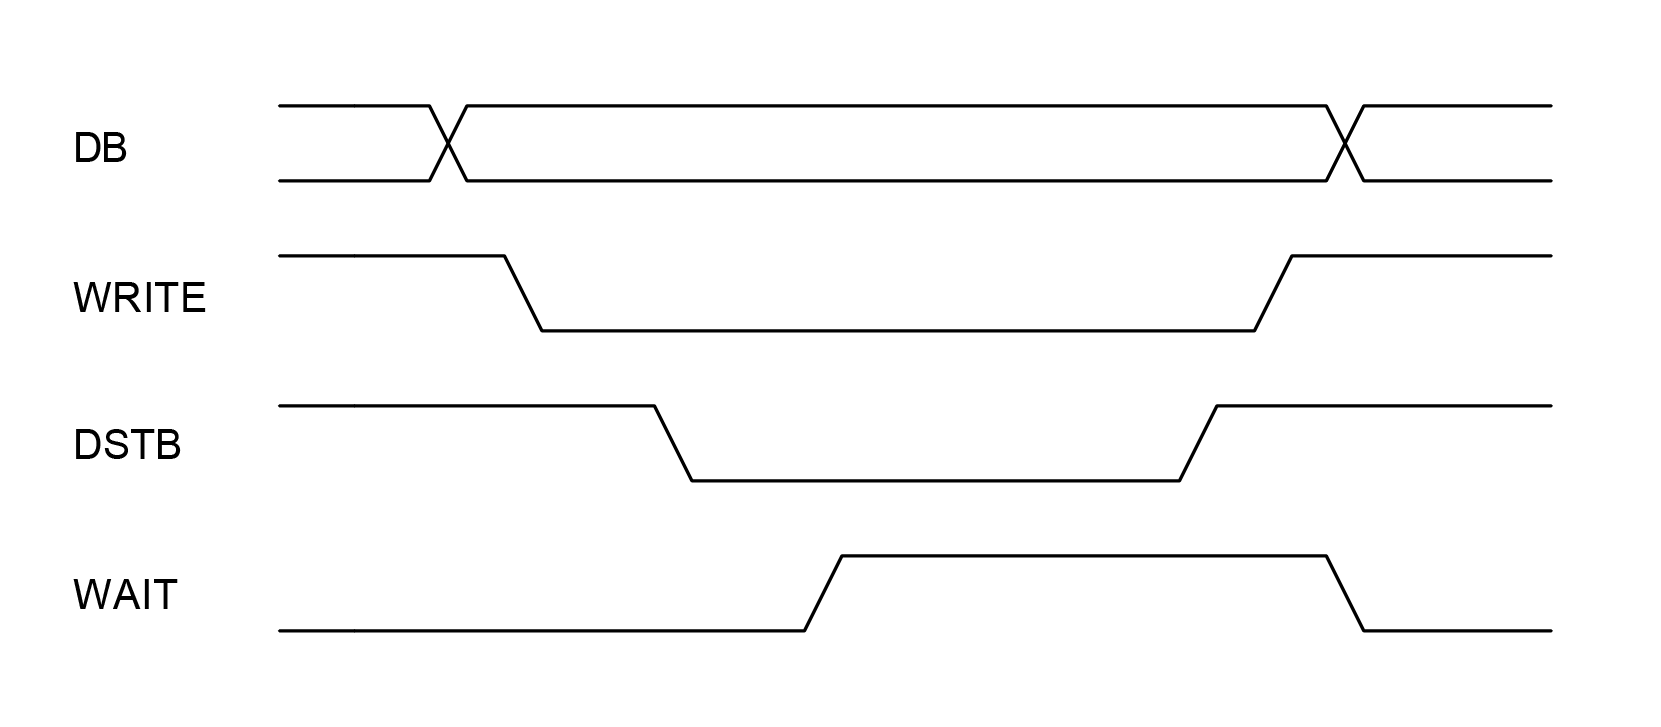
\includegraphics[width=0.4\textwidth]{figuras/data_write.png} 
	\caption{\label{data_write} Escritura de dato.}
	\end{center}
	\end{figure}

\hfill \break

La señal WRITE indica si la operación es de escritura(low) o de lectura(high). Las señales ASTB y DSTB indican si la operación es de dirección o de datos, solo una de estas dos puede estar activa(low) en todo momento. Por ultimo, la señal WAIT sirve para evitar colisiones e indica por parte de la FPGA que la aplicación esta ocupada en alguna operación.

 Con estas cuatro operaciones se implementan funciones de más alto nivel, de las cuales a nosotros nos interesan las de escritura y lectura de registros. La función de escritura se compone de una escritura de dirección seguido de una escritura de dato. Por otro lado la función de lectura se compone de una escritura de dirección seguido de una lectura de dato. Estas funciones son llevadas a cabo por el host nuestra tarea es implementar un driver en la FPGA que permita encargarse de estas desde el lado de la aplicación.
 
\section{Detalle de la aplicación}

La figura \ref{sistema_completo} entrega un diagrama del sistema a implementar para un caso general. En el sistema presentado en esta guía, la aplicación en la FPGA consiste en una memoria de dos puertos. Uno de estos puertos, el puerto A, quedará a disposición del host, mientras que el  puerto B quedara a disposición del usuario por medio de los periféricos disponibles en la tarjeta.

\begin{figure}[h!]
\begin{center}
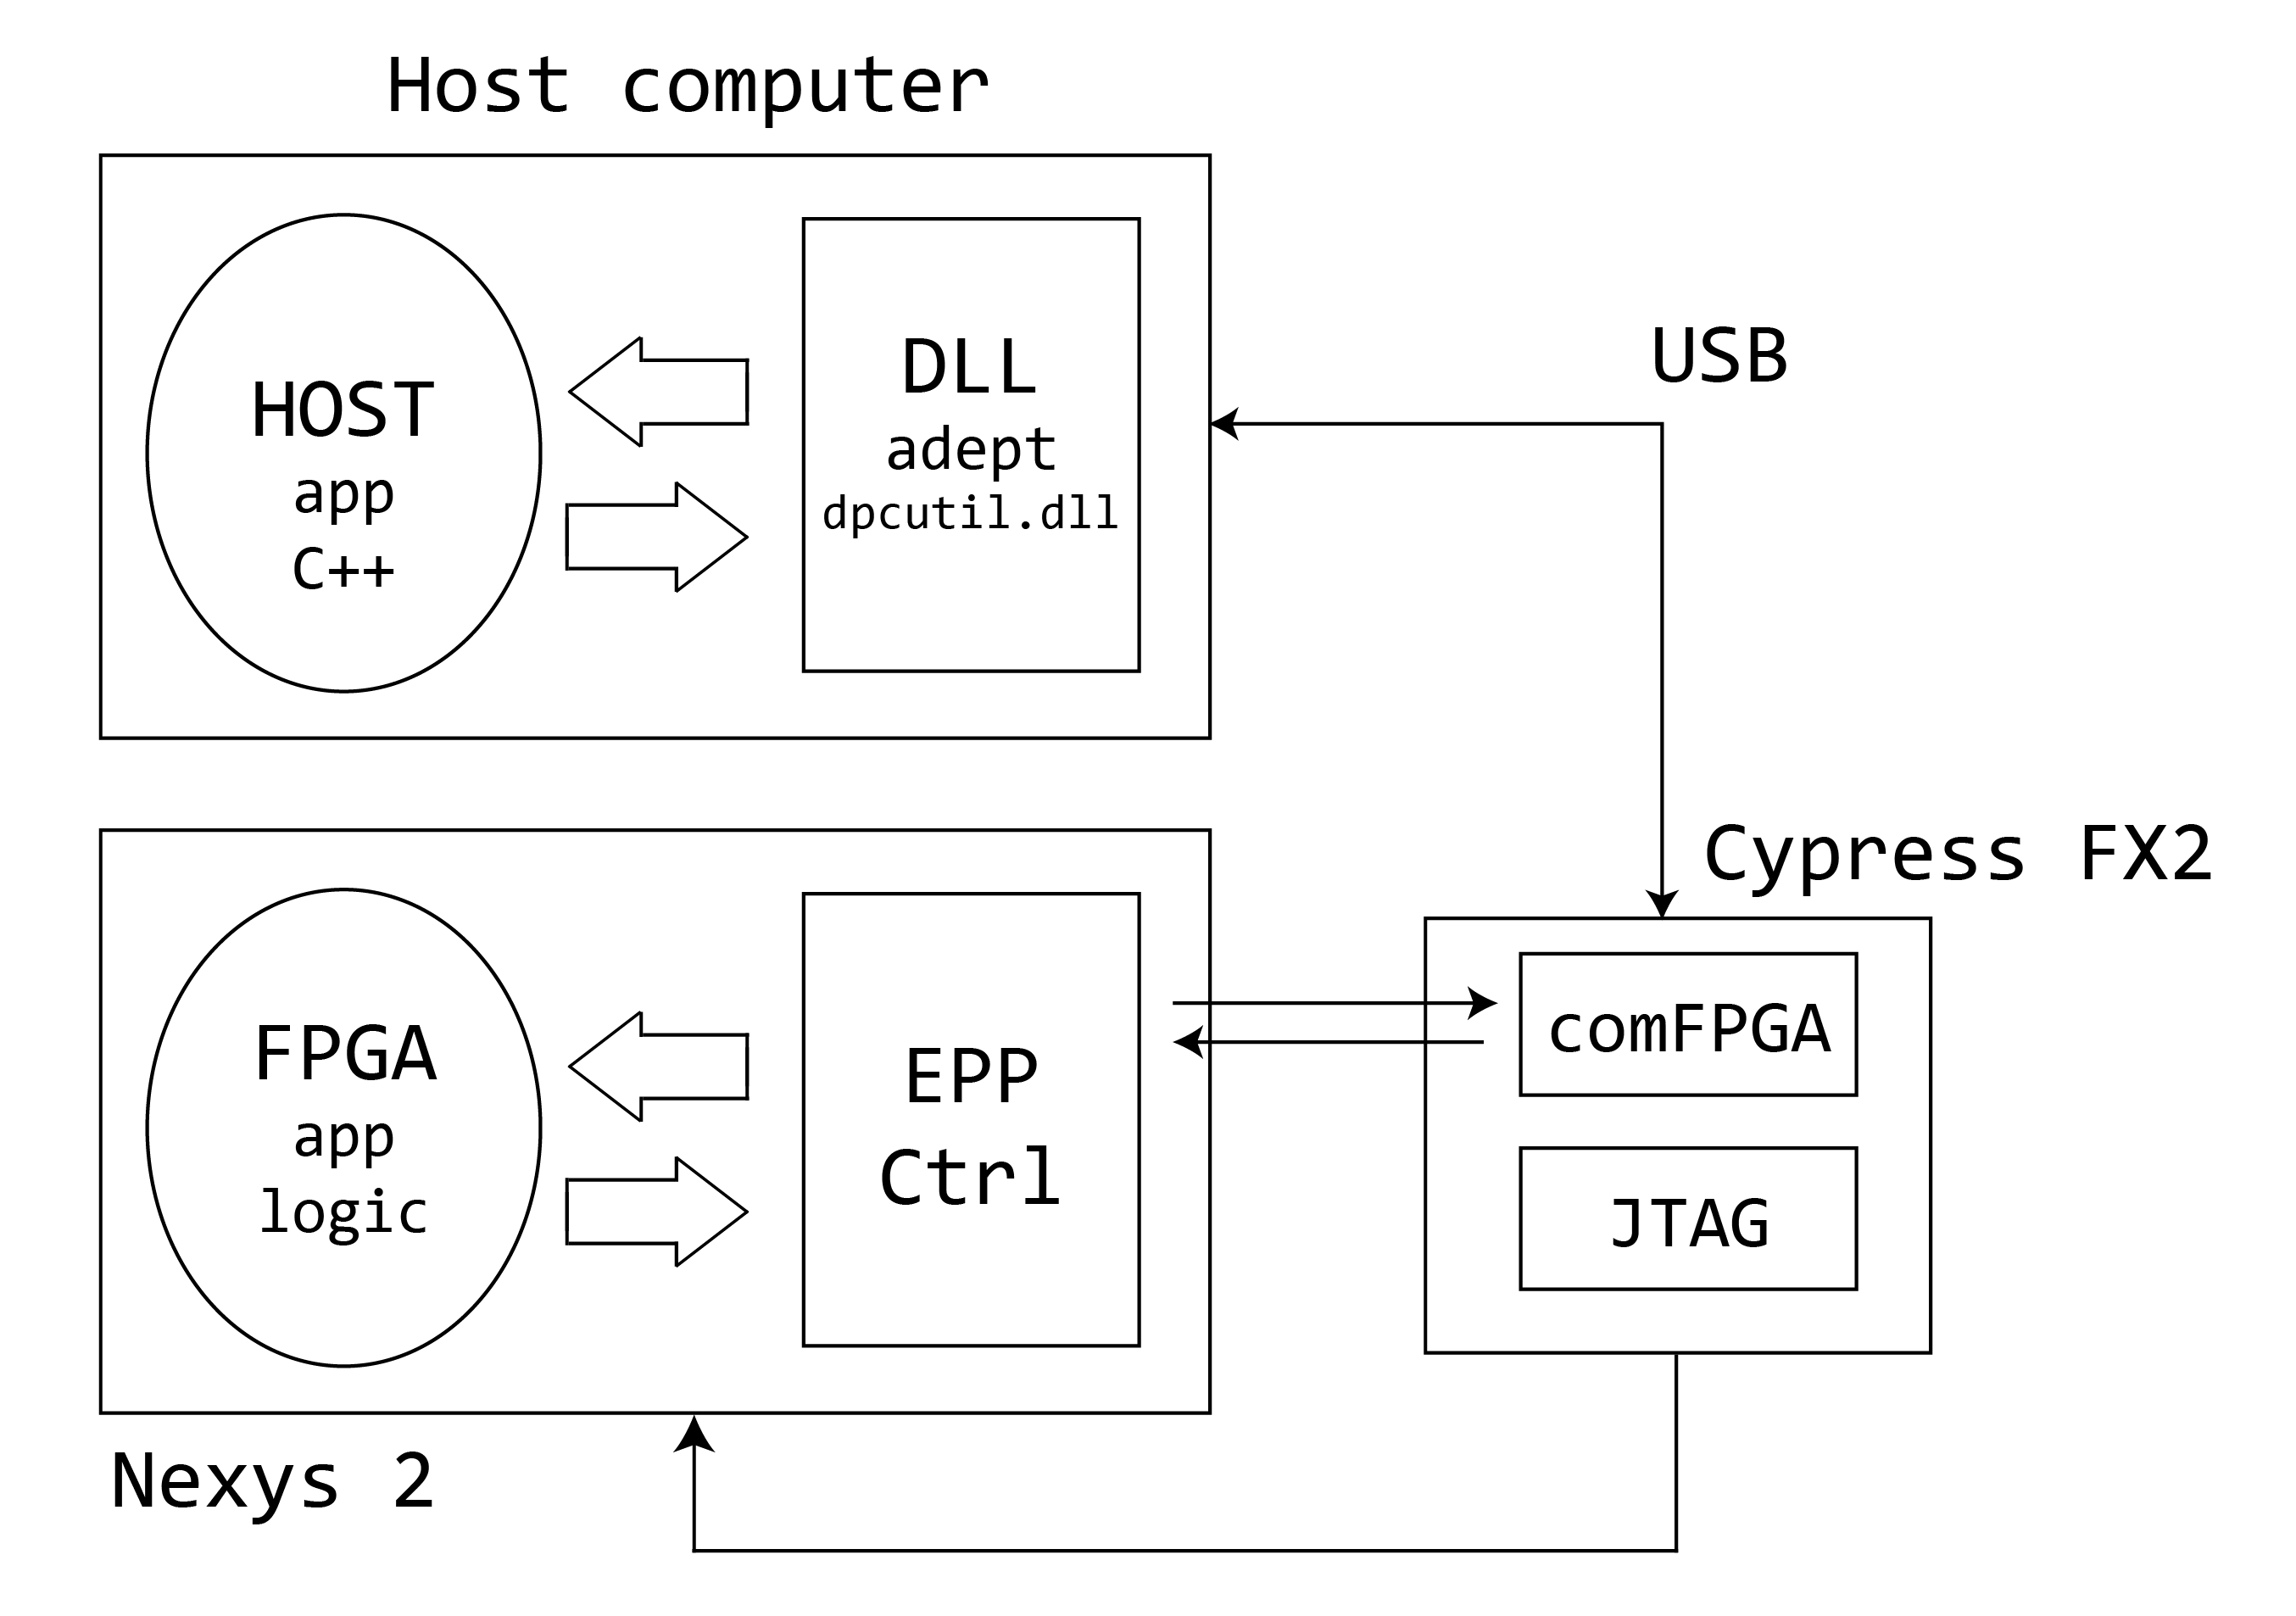
\includegraphics[scale=0.5]{figuras/sistema_total.png} 
\caption{\label{sistema_completo} Diagrama del sistema implementado. En este esquema el master es implementado por el host y el esclavo por la Nexys 2}
\end{center}
\end{figure}

 En las siguientes secciones explicaremos como implementar este sistema. En la sección \ref{sec5} se detalla el esclavo, el cual esta compuesto por el driver de la comunicación EPP\footnote{ Controlador capaz de llevar a cabo la comunicación entre el emulador de puerto paralelo y la aplicación en la FPGA.} y la aplicación en la FPGA. Por otro lado, en la sección \ref{sec6} se detalla la implementación del master, el cual esta compuesto por una aplicación en C++ en el computador, la cual se encarga de llamar a los drivers y controlar la comunicación con la tarjeta.


\section{Implementación del esclavo\label{sec5}}
La figura \ref{sistema_esclavo} presenta el diagrama de los bloques a implementar en la FPGA. Esta implementación cuenta con tres módulos, el primero solo es un driver para recibir las señales provenientes desde el host a través del emulador de puerto paralelo. El segundo módulo, BramComCtrl se encarga de interpretar estas señales y controlar la comunicación con la memoria, y por último tenemos la memoria de dos puertos. 

\begin{description}
\item[EppCtrl] Este módulo se encarga de lidiar con el tráfico de datos desde el puerto paralelo emulado hacia el resto de la aplicación. La comunicación esta controlada por tres señales \textbf{Write}, \textbf{Astb} y \textbf{Dstb}. Según estas señales el módulo se encarga de actualizar la dirección actual de la aplicación, actualizar los datos de entrada a la aplicación y actualizar los datos de salida hacia el emulador del puerto paralelo.
\item[BramComCtrl] A partir de las señales generadas en el módulo EppCtrl genera las señales necesarias para escribir o leer en la memoria. Este modulo es síncrono para evitar latchs.
\item[BRAMAB] Este bloque implementa una memoria de dos puertos. El puerto A es dedicado a la comunicación desde el host. Por otro lado, el puerto B queda a libre disposición para cualquier aplicación en la FPGA. En esta oportunidad simplemente podra ser accedida por medio de los switch y la salida del puerto será observable por los LEDS.
\end{description}


\begin{figure}[h!]
\begin{center}
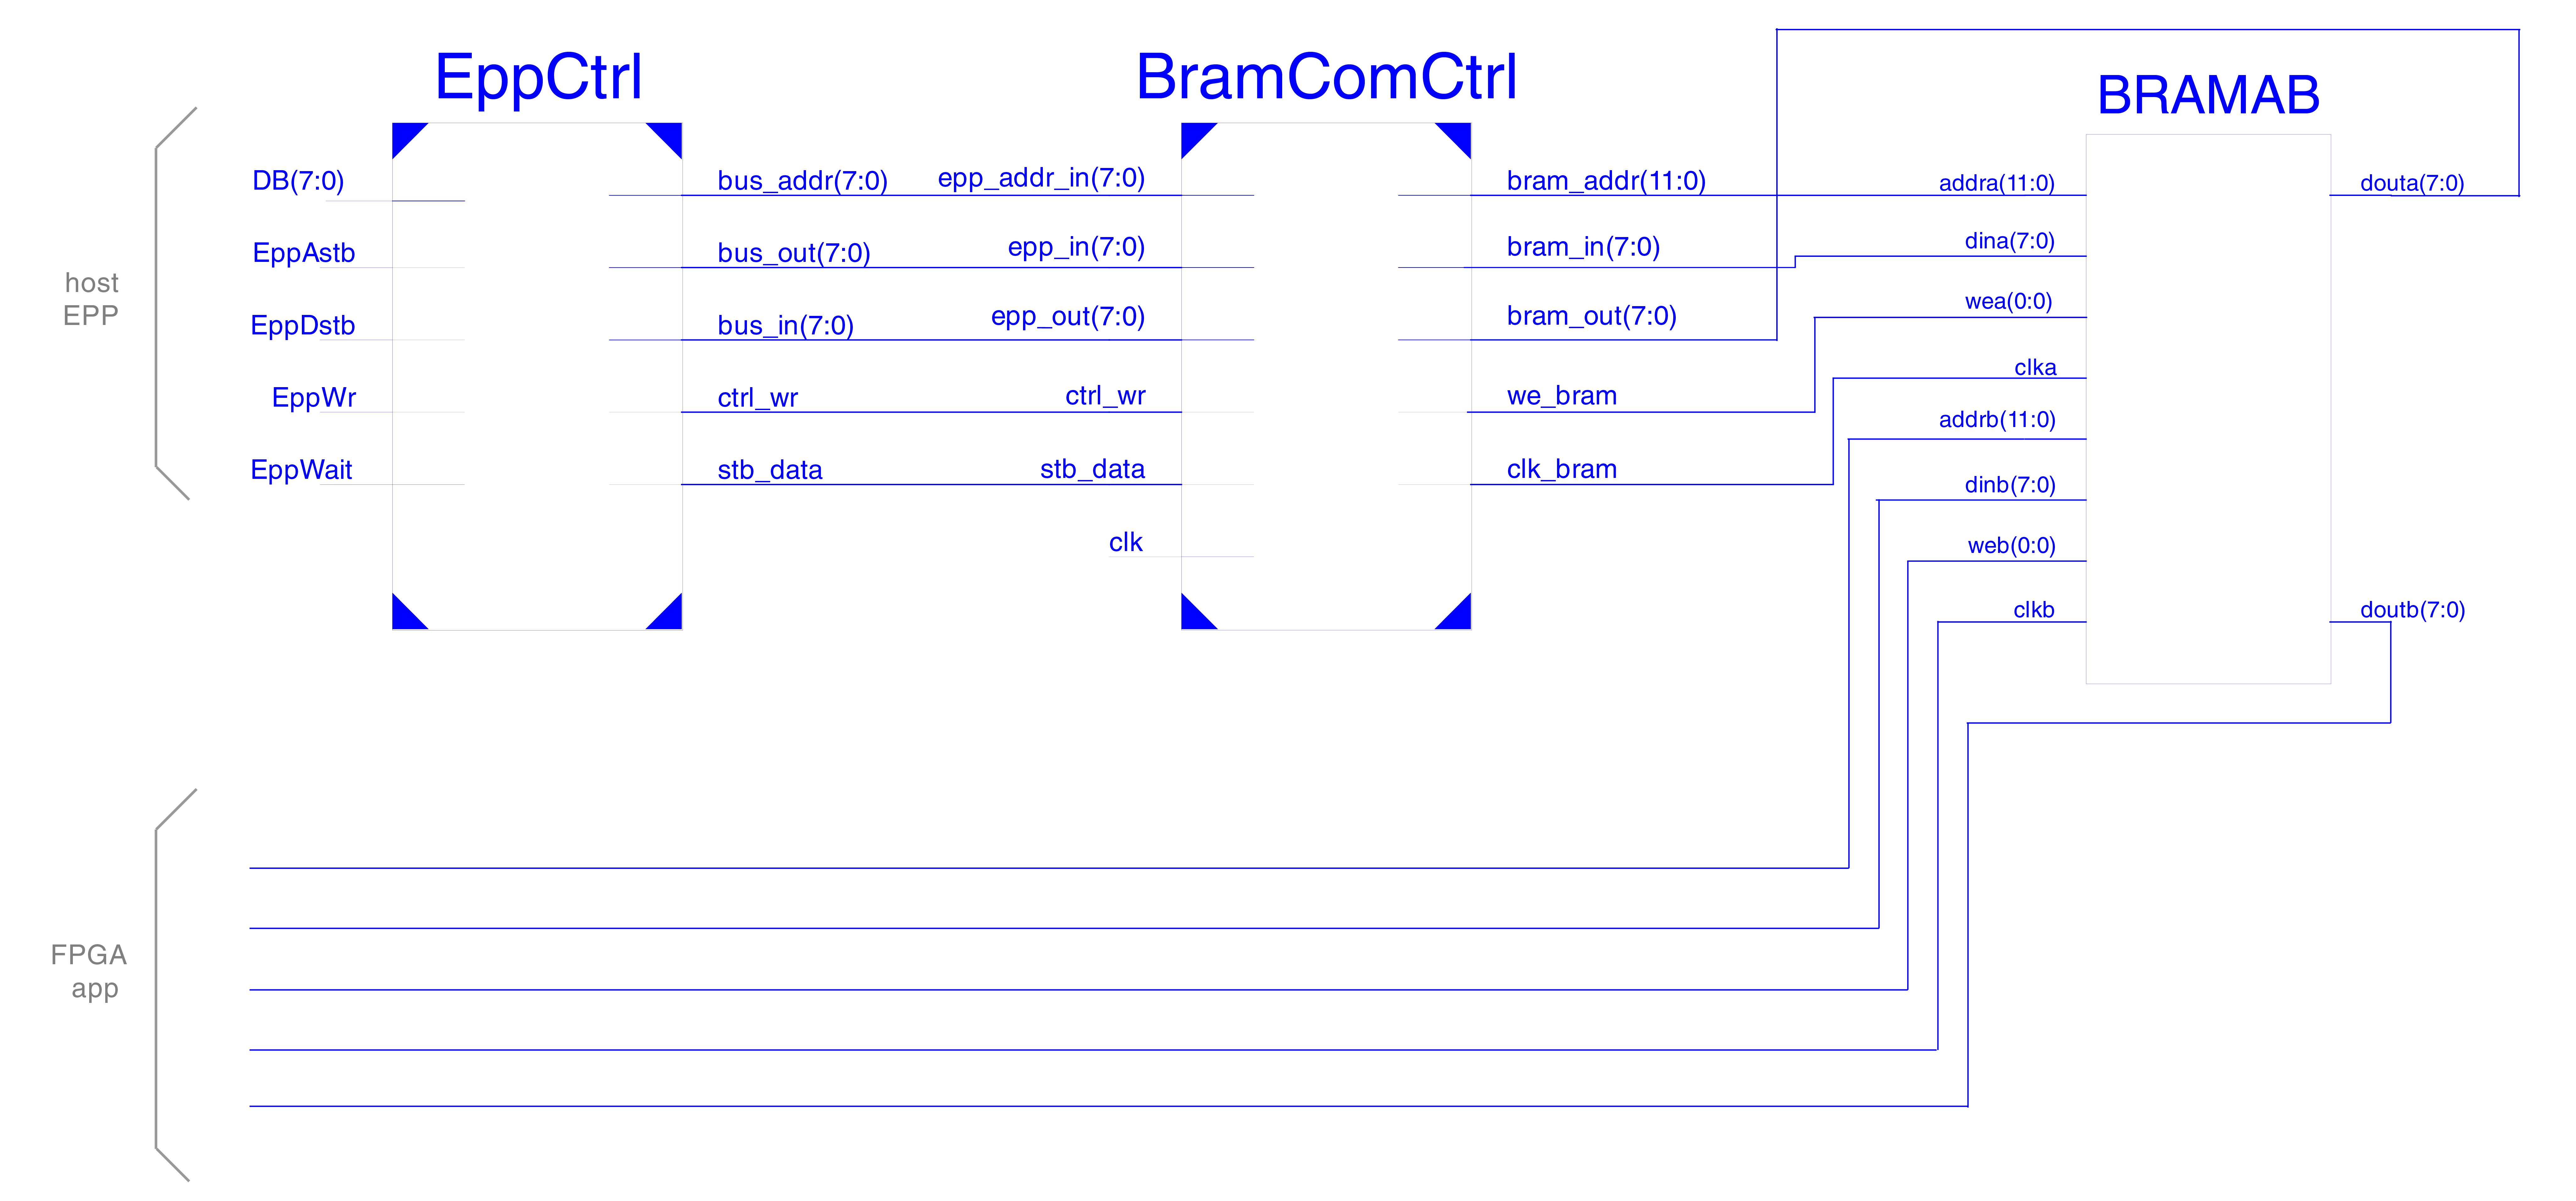
\includegraphics[width=0.8\textwidth]{figuras/figuras-04.png} 
\caption{\label{sistema_esclavo} Diagrama de los bloques implementados en la FPGA.}
\end{center}
\end{figure}

\section{Implementación del maestro\label{sec6}}
Para poder implementar correctamente el maestro, necesitamos desarrollar un programa que sea capaz de manipular la biblioteca  de funciones anteriormente mencionada. No existe una restricción sobre el lenguaje en el cual implementar dicho programa. En esta guía la aplicación fue desarrollada en $C++$ por medio del IDE Microsoft Visual 2010\footnote{IDE descargable de forma gratuita desde el sitio https://www.microsoft.com/es-cl/download}, en el cual crearemos una aplicación para consola.
El programa implementado utiliza básicamente 6 funciones entregadas por el fabricante\footnote{disponibles en https://reference.digilentinc.com/\_media/dpcutil\_programmers\_reference\_manual.pdf} las cuales se detallan a continuación

\begin{table}
\begin{center}
\begin{tabular}{|c|c|p{5cm}|p{5cm}|}
\hline 
Funcion & Salida & Entrada & Descripción \\ 
\hline 
DpcInit() & bool & Puntero a ERC & iniciliza los DLL. Debe ser llamada antes de cualquier otra función de la aplicación \\ 
\hline 
DpcOpenData() & bool & \begin{itemize}
\item Puntero para manipular la interfaz de datos.
\item Nombre del interfaz utilizad.
\item Puntero a un ERC. 
\item Null\footnote{esta funcionalidad no es de interés para la aplicación}
\end{itemize}  & Abre una interfaz de comunicación, es necesaria para utilizar cualquier otra de las funciones de comunicación  \\ 
\hline 
DpcCloseData() & bool & Puntero para manipular la interfaz de datos & Libera la interfaz de comunicación especificada y cierra el módulo de comunicación \\ 
\hline 
DpcTerm() & ninguno & ninguno & Termina el uso de los DLL cuando la aplicación es finalizada. \\ 
\hline 
DpcPutReg() & bool & Puntero para manipular la interfaz de datos, Variable BYTE con el registro dirección, Variable con el dato a enviar, puntero a un error, Null\footnote{esta funcionalidad no es de interés para la aplicación} & Envía el dato dado a la dirección especificada. \\ 
\hline 
DpcPutRegRepeat & bool & Puntero para manipular la interfaz de datos, Variable BYTE con el registro dirección, Puntero a un conjunto de Byte de datos a  enviar, puntero a un error, Null\footnote{esta funcionalidad no es de interés para la aplicación}  & Envía un conjunto de datos a una única dirección \\ 
\hline 
\end{tabular} 
\end{center}
\end{table}


\subsection{Incluir \textit{headers} y bibliotecas}
Para poder llamar correctamente a las funciones entregadas por el fabricante, debemos incluir los headers y las bibliotecas disponibles en el SDK \footnote{https://reference.digilentinc.com/digilent\_adept\_2}. Los headers que utilizaremos en nuestro programa son 
\begin{itemize}
\item dpcdec1.h
\item depp.h
\item dmgr.h
\item dpcutil.h
\item dpcdefs.h
\end{itemize}
Estos deben agregarse a nuestro directorio de trabajo del proyecto y posteriormente agregarlos al programa utilizando \verb+add/from existing item+ desde nuestra carpeta de \verb+headers file+.

Luego debemos agregar las bibliotecas a nuestro programa, para esto debemos copiar la carpeta \verb+lib+, disponible en los SDK del fabricante, a nuestro directorio de trabajo. Una vez hecho esto, debemos ir a \verb+Proyect/Properties+ buscar la opción \verb+Configuration Properties/Linker+ y agregar la carpeta \verb+lib+ en la línea \verb+Additional Library Directories+. 
Finalmente dentro de la misma pantalla de \verb+Configuration Properties/Linker+ debemos ir la opción \verb+Input+ y en la línea \verb+Additional Dependencies+ debemos agregar las siguientes bibliotecas.

\begin{itemize}
\item dpcomm.lib
\item depp.lib
\item dmgr.lib
\item dpcutil.lib
\end{itemize}




\end{document}
